\section{Auswertung}
\label{sec:auswertung}

\section{Fehlerrechnung}
\label{subsec:fehlerrechnung}

\subsubsection{Mittelwert}
\begin{equation}
\overline{v} = \frac{1}{N} \sum_{i=1}^N v_i
\end{equation}

\subsubsection{Standardabweichung}
\begin{equation}
s_i = \sqrt{\frac{1}{N - 1} \sum_{j=1}^N \left(v_j - \overline{v}\right){^2}}
\end{equation}

wobei $v_j$ ($j = 1, ..., N$) die Messwerte sind.

\subsubsection{Streuung der Mittelwerte}
\begin{equation}
\sigma_i = \frac{s_i}{\sqrt{N}} = \sqrt{\frac{\sum_{j=1}^N \left(v_j - \overline{v_i}\right){^2}}{N \left(N - 1 \right)}}
\end{equation}

\subsubsection{Gaußfehler}
Bei einer fehlerbehafteten Funktion $f$ mit $k$ als fehlerbehafteter Größe und $\sigma_k$ als Ungenauigkeit, gilt:

\begin{equation}
\Delta x_k = \frac{\mathrm{d}f}{\mathrm{d}k}\sigma_k
\end{equation}.

 Der relative Gaußfehler berechnet sich nach:
\begin{equation}
\Delta x_\text{k, rel} = 1 \pm \frac{\Delta x_k}{|x|}\cdot 100\%
\end{equation}.

Der absolute Gaußfehler ergibt sich aus:
\begin{equation}
\Delta x_i = \sqrt{\left(\frac{\mathrm{d}f}{\mathrm{d}k_{1}}\cdot \sigma_{k_{1}}\right)^2 + \left(\frac{\mathrm{d}f}{\mathrm{d}k_{2}}\cdot \sigma_{k_{2}}\right)^2 + ...}
\end{equation}.


\subsection{Güteziffer}
  \label{subsec:güteziffer}
  Es soll die reale Güteziffer der Wärmepumpe ermittelt werden. Diese ergibt sich nach (\ref{eqn:güteziffer1}) und (\ref{eqn:güteziffer2}) zu
  \begin{equation}
    ν = \frac{(m_{1} c_w + m_k c_k)}{N}\frac {\mathrm{d}T_{1}}{\mathrm{d}t}.
  \end{equation}
  Der dort auftretende Differentialquotient $\frac {\mathrm{d}T_{1}}{\mathrm{d}t}$ lässt sich durch einen Fit der Messdaten an eine Funktion der Form
  \begin{equation}
    T(t) = A t^2 + Bt + C
  \end{equation}
  errechnen. Die Messdaten ergeben die in Tabelle \ref{tab:koeffizienten} angegebenen Koeffizienten (von Einheiten wurde mangels physikalischen Sinns abgesehen):

  \begin{table}[!h]
    \centering
    \caption{Koeffizienten des nichtlinearen Fits.}
    \label{tab:koeffizienten}
    \sisetup{
      round-mode=figures,
      round-precision=3,
    }
    \begin{tabular}{
        c
        S[table-format=1.2e2] @{${}\pm{}$} S[table-format=1.2e2]
        S[table-format=1.2e2] @{${}\pm{}$} S[table-format=1.2e2]
        S[table-format=1.2e1] @{${}\pm{}$} S[table-format=1.2e2]}
      \toprule
      Messpunkt & \multicolumn{2}{c}{$A / \si{\kelvin\per\second\squared}$}
      & \multicolumn{2}{c}{$B / \si{\kelvin\per\second}$}
      & \multicolumn{2}{c}{$C / \si{\kelvin}$}\\
      \midrule
      $T_1$
      \input{coefficients1.tex}
      $T_2$
      \input{coefficients2.tex}
      \bottomrule
    \end{tabular}
  \end{table}
  Mithilfe der zeitlichen Ableitung von $T(t)$
  \begin{equation}
    \frac{\mathrm{d}T(t)}{\mathrm{d}t} = 2At + B
  \end{equation}
  und der Wärmekapazität
  \begin{align}
    c_w = \SI{4.2 +- 0.04}{\kilo\joule\per\kilogram\per\kelvin},
  \end{align}
  sowie Dichte von Wasser
  \begin{align}
    \rho = \SI{994(10)}{\kilogram\per\meter\cubed},
  \end{align}
  deren Wert nach \cite[Dba2]{wärmeatlas} im relevanten Temperaturbereich gemittelt wurden, des Volumen des Wassers im Reservoir
  \begin{align}
    V = \SI{4000 +- 0.4}{\milli\liter},
  \end{align}
  der daraus resultierenden Masse des Wassers
  \begin{align}
    m_1 = \SI{4.0+-0.4}{\kilogram},
  \end{align}
  und damit Wärmekapazität
  \begin{align}
    C = \SI{1.67(17)e4}{\joule\per\kelvin}
  \end{align}
   und der angegebenen Wärmekapazität der Apparatur
  \begin{align}
    c_km_k = \SI{750(10)}{\joule\per\kelvin}
  \end{align}
  kann dann die Güteziffer zu verschiedenen Zeitpunkten ermittelt werden.

  Im Vergleich dazu sollte nach (\ref{eqn:güte_ideal}) zu den selben Zeitpunkten die Güteziffer einer idealen Wärmepumpe ermittelt werden, die bei den entsprechenden Temperaturniveaus arbeitet. Der Fehler für diese Größe wird mit
  \begin{equation}
    \Delta \nu_\mathrm{ideal} = \sqrt{\frac{1}{(T_1-T_2)^4} \cdot (T_2^2 \Delta T_1^2 + T_1^2 \Delta T_2^2)}
  \end{equation}
  bestimmt.
  Die Ergebnisse sind Tabelle \ref{tab:ergebnisse_güte} und Abb. \ref{fig:temperatur} zu entnehmen, wobei der Fehler der realen Güteziffer
  \begin{align}
    (\Delta \nu_\mathrm{real})^2 &= \frac{1}{N^2}((c_w \dot{T}_1 V \Delta \rho)^2 + (c_w \rho \dot{T}_1 \Delta V)^2 \\
    &\quad + (\rho \dot{T}_1 V \Delta c_w)^2 + (\dot{T}_1 \Delta C)^2 \\ &\quad + ((c_w \rho V + C) \Delta \dot{T}_1)^2)
  \end{align}
  \begin{align}
  \intertext{mit}
    m_k c_k &= C
  \intertext{und}
    \frac{\mathrm{d}T_1(t)}{\mathrm{d}t} &= \dot{T}_1
  \end{align}
  \begin{table}[h]
    \centering
    \caption{Ermittelte Gütezahlen.}
    \label{tab:ergebnisse_güte}
    \sisetup{
      round-mode=figures,
      round-precision=3,
    }
    \begin{tabular}{
        l@{}
        S[table-format=4.0]
        S[table-format=3.0] @{${}\pm{}$} S[table-format=2.1]
        S[table-format=1.2] @{${}\pm{}$} S[table-format=1.3]
        S[table-format=2.2] @{${}\pm{}$} S[table-format=1.5]
        S[table-format=1.4] @{${}\pm{}$} S[table-format=1.5]}
      \toprule
      & $t / \si{\second}$
      & \multicolumn{2}{c}{$\sfrac{\mathrm{d}T}{\mathrm{d}t} / \si{\kelvin\per\second}$}
      & \multicolumn{2}{c}{$ν_{\mathrm{real}}$}
      & \multicolumn{2}{c}{$ν_{\mathrm{ideal}}$}
      & \multicolumn{2}{c}{$ν_{\mathrm{real}} / ν_{\mathrm{ideal}}$} \\
      %& \multicolumn{2}{c}{$\dot m / \si{\gram\per\second}$}
      %& \multicolumn{2}{c}{$N / \si{\watt}$} \\
      \midrule
      \input{table_guete.tex}
      \bottomrule
    \end{tabular}
  \end{table}

  \begin{figure}[htpb]
    \centering
    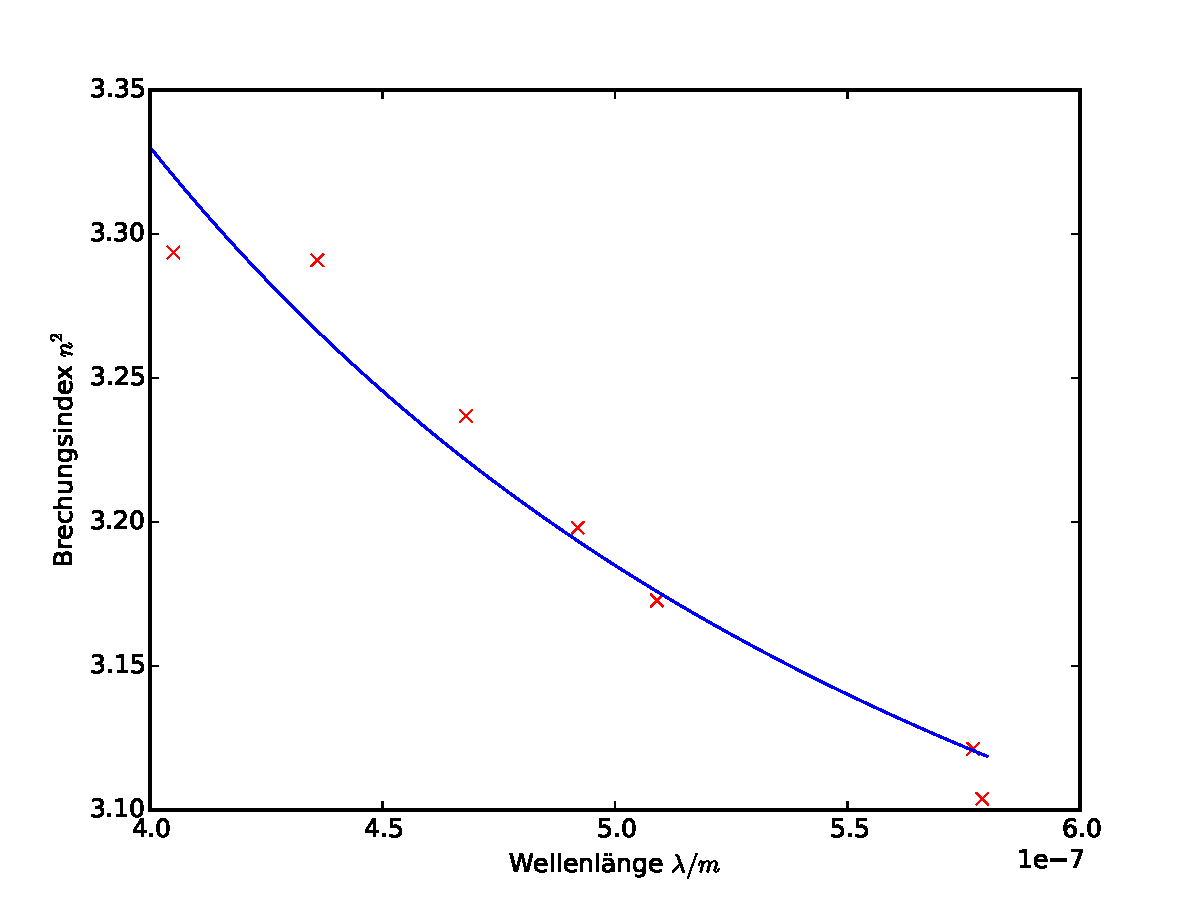
\includegraphics{plot.pdf}
    \caption{Plot des Temperaturverlaufs und der Fits. Auf Fehlerbalken wurde zwecks verbesserter Lesbarkeit verzichtet.}
    \label{fig:temperatur}
  \end{figure}

\newpage
\subsection{Massendurchsatz}
  Außerdem soll der Massendurchsatz des Kreislaufes ermittelt werden. Dies geschieht, indem (\ref{eqn:durchsatz1}) und (\ref{eqn:durchsatz2}) zu
  \begin{equation}
    \frac{\mathrm{d}m}{\mathrm{d}t} = \dot m = \frac{(m_{2} c_w + m_k c_k)}{L}\frac {\mathrm{d}T_{2}}{\mathrm{d}t}
  \end{equation}
  umgestellt werden. Der Differentialquotient $\frac {\mathrm{d}T_{2}}{\mathrm{d}t}$ wird exakt wie in Abschnitt \ref{subsec:güteziffer} mittels nichtlinearer Ausgleichsrechnung bestimmt. Die Fehlerformel für $\dot m$ lautet
  \begin{align}
    (\Delta \dot m)^2 &= \frac{1}{L^2}((c_w \dot{T}_2 V \Delta \rho)^2 + (c_w \rho \dot{T}_2 \Delta V)^2 \\
    &\quad + (\rho \dot{T}_2 V \Delta c_w)^2 + (\dot{T}_2 \Delta C)^2 \\ &\quad + ((c_w \rho V + C) \Delta \dot{T}_2)^2).
  \end{align}
  Die Verdampfungswärme $L$ lässt sich aus der (vom Manometer abgelesenen) Dampfdruckkurve von Dichlordifluormethan (Tabelle \ref{tab:dampfdruck}) mithilfe einer linearen Regression des logarithmierten Drucks über die reziproke Temperatur ermitteln. Nach \cite{anleitung203} gilt folgende Näherung der Clausius-Clapeyron-Gleichung für Temperaturen $T \ll T_\mathrm{kritisch}$:
  \begin{equation}
    \ln p = -\frac{L}{R} \frac {1}{T} + \mathrm{const.}
  \end{equation}
  Damit ergibt sich
  \begin{equation}
    L = -R \cdot a
  \end{equation}
  mit der Steigung $a$ der Ausgleichsgeraden und der universellen Gaskonstante
  \begin{equation}
    R = \SI[separate-uncertainty=false]{8.3144598(48)}{\joule\per\mol\per\kelvin}
  \end{equation}
  \cite{codata}. Die Gaußsche Fehlerformel für $L$ ist damit
  \begin{equation}
    \Delta L = \sqrt{a^2 (\Delta R)^2 + R^2 (\Delta a)^2}
  \end{equation}
  Der Durchsatz in \si{\mol\per\second} wird noch mit der molaren Masse
  \begin{equation}
    M = \SI{120.913}{\gram\per\mol}
  \end{equation}
  \cite[267]{gase} des Kältemittels multipliziert um nicht nur die Anzahl der Moleküle, sondern die Masse zu erhalten. Eine grafische Darstellung der Dampfdruckkurve findet sich in Abb. \ref {fig:dampfdruck}, das Ergebnis für die Verdampfungswärme in Tabelle \ref{tab:ergebnis_L}, die Ergebnisse für den Massendurchsatz in Tabelle \ref{tab:ergebnisse_durchsatz}, wobei das negative Vorzeichen, welches die \enquote{Flussrichtung} der Masse bestimmt, ignoriert wird.

  \begin{table}[htbp]
    \centering
    \caption{Ermittelte Steigung und Verdampfungswärme.}
    \label{tab:ergebnis_L}
    \sisetup{
      round-mode=figures,
      round-precision=4,
    }
    \begin{tabular}{
        l@{}
        S[table-format=4.0] @{${}\pm{}$} S[table-format=1.4]
        S[table-format=5.0, round-precision=5] @{${}\pm{}$} S[table-format=2.1, round-precision=3]}
      \toprule
      & \multicolumn{2}{c}{$ a / \si{\kelvin}$}
      & \multicolumn{2}{c}{$ L / \si{\joule\per\mol}$} \\
      \midrule
      \input{table_verdampfungswärme.tex}
      \bottomrule
    \end{tabular}
  \end{table}

  \begin{table}[htbp]
    \centering
    \caption{Ermittelte Massendurchsätze.}
    \label{tab:ergebnisse_durchsatz}
    \sisetup{
      round-mode=figures,
      round-precision=3,
    }
    \begin{tabular}{
        l@{}
        S[table-format=4.0]
        S[table-format=1.3] @{${}\pm{}$} S[table-format=1.4]}
      \toprule
      & $t / \si{\second}$
      & \multicolumn{2}{c}{$\dot m / \si{\gram\per\second}$} \\
      \midrule
      \input{table_massendurchsatz.tex}
      \bottomrule
    \end{tabular}
  \end{table}

  \begin{figure}[htpb]
    \centering
    \includegraphics{plot_dampfdruck.pdf}
    \caption{Plot der Dampfdruckkurve.}
    \label{fig:dampfdruck}
  \end{figure}

  \begin{table}[htbp]
    \centering
    \caption{Dampfdruckkurve von Dichlordifluormethan.}
    \label{tab:dampfdruck}
    \begin{subtable}{.49\textwidth}
      \centering
      \begin{tabular}{
          S[table-format=3.2]
          S[table-format=4.0]
        }
        \toprule
        $T / \si{\kelvin}$
        & $p/ \si{\kilo\pascal}$\\
        \midrule
         259.15 & 200 \\
         272.15 & 300 \\
         281.15 & 400 \\
         289.15 & 500 \\
         295.15 & 600 \\
         300.15 & 700 \\
         306.15 & 800 \\
         311.15 & 900 \\
         315.15 & 1000 \\
         319.15 & 1100 \\
         323.15 & 1200 \\
         327.15 & 1300 \\
         329.15 & 1400 \\
         332.15 & 1500 \\
         336.15 & 1600 \\
        \bottomrule
      \end{tabular}
    \end{subtable}
    \begin{subtable}{.49\textwidth}
      \centering
      \begin{tabular}{
          S[table-format=3.2]
          S[table-format=4.0]
        }
        \toprule
        $T / \si{\kelvin}$
        & $p/ \si{\kilo\pascal}$\\
        \midrule
        338.15 & 1700 \\
        340.15 & 1800 \\
        343.15 & 1900 \\
        345.15 & 2000 \\
        348.15 & 2100 \\
        350.15 & 2200 \\
        353.15 & 2300 \\
        355.15 & 2400 \\
        358.15 & 2500 \\
        360.15 & 2600 \\
        362.15 & 2700 \\
        365.15 & 2800 \\
        368.15 & 2900 \\
        369.15 & 3000 \\
        370.15 & 3100 \\
        \bottomrule
      \end{tabular}
    \end{subtable}
  \end{table}

\newpage
\subsection{Mechanische Kompressorleistung}
  Zuletzt soll die mechanische Leistung des Kompressors ermittelt werden. Diese ist nach (\ref{eqn:mechleistung})
  \begin{equation}
    N_\mathrm{mech} = \frac{1}{\kappa-1}\biggl(p_b \sqrt[\kappa]{\frac{p_a}{p_b}}-p_a\biggr)\frac{1}{\rho} \frac{\mathrm{d}m} {\mathrm{d}t}.
  \end{equation}
  Die Messunsicherheit beträgt
  \begin{align}
    (\Delta N_\mathrm{mech})²
    &= \left(\frac{1}{\kappa - 1}\left(p_b \sqrt[\kappa]{\frac{p_a}{p_b}} - p_a\right) \frac{1}{\rho} \Delta \dot m \right)² \\
    &\quad + \left(\frac{1}{\kappa - 1}\left(p_b \sqrt[\kappa]{\frac{p_a}{p_b}} - p_a\right) \frac{1}{\rho^2} \dot m \Delta \rho \right)² \\
    &\quad + \left(\frac{1}{\kappa - 1} \frac{1}{\rho} \dot m \left(\left(\frac{p_a}{p_b}\right)^{\sfrac{1}{\kappa}-1} -1 \right) \Delta p_a\right)² \\ &\quad + \left(\frac{1}{\kappa - 1} \frac{1}{\rho} \dot m \left(\sqrt[\kappa]{\frac{p_a}{p_b}} - p_a \left(\frac{p_a}{p_b}\right)^{\sfrac{1}{\kappa} - 1}\right) \Delta p_b \right)²
  \end{align}
  Die Dichte $\rho$ ist mithilfe der allgemeinen Gasgleichung zu bestimmen:

  \begin{align}
    pV &=nRT \\
    \Leftrightarrow \frac{pV}{T} &= nR
    \intertext{Im geschlossenen System gilt: $nR = \mathrm{const.}$ Also ist }
    \frac{p_0 V_0}{T_0} &= \frac{p_2 V_2}{T_2}
    \intertext{mit $V = \frac{m}{\rho}$ folgt}
    \frac{p_0 m_0}{\rho_0 T_0} &= \frac{p_2 m_2}{\rho_2 T_2},
    \intertext{da $m_0 = m_2$ ergibt sich}
    \frac{p_0}{\rho_0 T_0} = \frac{p_2}{T_2 \rho_2} &\Leftrightarrow \rho_2 = \frac{\rho_0 T_0 p_2}{T_2 p_0}
    \intertext{mit $\rho_{2} = \rho$ und $p_{2} = p_a$ also}
    \rho &= \frac {\rho_0 T_0 p_a}{T_2 p_0}
  \end{align}
  \begin{align}
    \intertext{damit folgt für die Messunsicherheit}
    \Delta \rho &= \sqrt{\left(\frac{\rho_0 T_0}{T_2 p_0} \Delta p_a\right)² + \left(\frac{\rho_0 T_0 p_a}{p_0 T_2^2} \Delta T_2\right)²}
  \end{align}

  In der Versuchsanleitung\cite{anleitung206} sind die Werte
  \begin{align}
    \rho_{0} &= \SI{5.51}{\gram\per\liter},\\
    p_{0} &= \SI{1}{\bar},\\
    T_{0} &= \SI{0}{\celsius},\\
    \kappa &= \num{1.14}
  \end{align}
  gegeben, die restlichen Größen werden den Messdaten entnommen. Die berechneten mechanischen Kompressorleistungen finden sich in Tabelle \ref{tab:ergebnisse_leistung}.

  \begin{table}[htpb]
    \centering
    \caption{Ermittelte Leistungen.}
    \label{tab:ergebnisse_leistung}
    \sisetup{
      round-mode=figures,
      round-precision=3,
    }
    \begin{tabular}{
        l@{}
        S[table-format=4.0]
        S[table-format=2.1] @{${}\pm{}$} S[table-format=1.2]
        S[table-format=2.2] @{${}\pm{}$} S[table-format=1.2]}
      \toprule
      & $t / \si{\second}$
      & \multicolumn{2}{c}{$\rho / \si{\kilo\gram\per\meter\cubed}$}
      & \multicolumn{2}{c}{$N_{\mathrm{mech}} / \si{\watt}$} \\
      \midrule
      \input{table_kompressorleistung.tex}
      \bottomrule
    \end{tabular}
  \end{table}

  \newgeometry{top=3cm, bottom=5cm}
  \subsection{Messdaten}
  \begin{table}[htpb]
    \tiny
    \centering
    \caption{Messdaten.}
    \label{tab:messdaten}
    \begin{tabular}{l@{}
        S[table-format=4.0]
        S[table-format=3.2]
        S[table-format=3.2]
        S[table-format=3.0]
        S[table-format=4.0]
        S[table-format=3.0]
      }
      \toprule
      & $t / \si{\second}$
      & $T_{1} / \si{\kelvin}$
      & $T_{2} / \si{\kelvin}$
      & $p_a / \si{\kilo\pascal}$
      & $p_b / \si{\kilo\pascal}$
      & $P / \si{\watt}$ \\
      \midrule
      \input{table_data.tex}
      \midrule
      \multicolumn{7}{c}{Messunsicherheiten:}\\
      \multicolumn{7}{c}{$\Delta T = \SI{0.1}{\kelvin}, \Delta p_a = \SI{0.2}{\bar}, \Delta p_b = \SI{1}{\bar}, \Delta V = \SI{0.4}{\milli\liter}$}\\
      \bottomrule
    \end{tabular}
  \end{table}
  \restoregeometry
